Many of today's well-known salient object algorithms have the following two components: 1) a suitable representation for salient object segmentation, and 2) computational principles of feature saliency, such as region contrast \cite{cheng2011global} or element uniqueness \cite{perazzi2012saliency}.  However, none of these two components alone is new to computer vision.  On one hand, detecting boundaries of objects has been a highly desired goal for segmentation algorithms since the beginning of computer vision  On the other hand, defining rules of saliency has been studied in fixation analysis for decades.  In this section, we build a salient object segmentation model by combining existing techniques of segmentation and fixation based saliency. The core idea is to first generate a set of object candidates, and then use the fixation algorithm to rank different regions based on their saliency. This simple combination results in a novel salient object segmentation method that outperforms \emph{all} previous methods by a large margin.

\subsection{Salient object, object proposal and fixations}
Our first step is to generate the segmentation of object candidates by a generic object proposal method. We use CPMC \cite{carreira2010constrained} to obtain the initial segmentations. CPMC is an unsupervised framework to generate and rank plausible hypotheses of object candidates without category specific knowledge. This method initializes foreground seeds uniformly over the image and solves a set of min-cut problems with different parameters. The output is a pool of object candidates as overlapping figure-ground segments, together with their ``objectness'' scores. The goal of CPMC is to produce a over-complete coverage of potential objects, which could be further used for tasks such as object recognition.

The representation of CPMC-like object proposal is easily adapted to salient object segmentation.  If all salient objects can be found from the pool of object candidates, we can reduce the problem of salient object detection to a much easier problem of salient segment ranking. Ranking the segments also simplifies the post-processing step. As the segments already preserve the boundary of the image, no explicit segmentation (e.g.\ GraphCut~\cite{cheng2011global}) is required to obtain the final binary object mask.

To estimate the saliency of a candidate segment, we utilize the spatial distribution of fixations within the object.  It is well known that the density of fixation directly reveals the saliency of the segment.  The non-uniform spatial distribution of fixations on the object also offers useful cues to determine the saliency of an object. For example, fixation at the center of a segment will increase its probability of being an object.  To keep our frame work simple, we do not consider class specific or subject specific fixation patterns in our model.

\subsection{The model}
We use a learning based framework for the segment selection process. This is achieved by learning a scoring function for each object candidate. Given a proposed object candidate mask and its fixation map, this function estimates the overlapping score (intersection over union) of the region with respect to the ground-truth, similar to~\cite{li2010object}.

\textbf{Features:} We extract two types of features: shape features and fixation distribution features within the object. The shape features characterizes the binary mask of the segment, which includes major axis length, eccentricity, minor axis length, and the Euler number. For fixation distribution features, we first align the major axis of each object candidate, and then extract a $4\times3$ histogram of fixations density over the aligned object mask. This histogram captures the spatial distribution of the fixations within a object.

Without loss of generality, we use the term {\it fixation energy} to refer to pixel values in the fixation map. For human fixations, the energy is a discrete value as the number of fixations at current location. For algorithm generated fixation maps, the energy is a continuous value ranging from $0$ to $1$ as the probability of a fixation at current location. Finally, the $33$ dimensional feature vector is extracted for each object mask. The details of the features can be found in Table.~\ref{tab:feat}.  In particular, the {\it Fixation Energy Ratio} is the defined as the sum of fixation energy within the segment, divided by the sum of fixation energy of the whole image.

\begin{table}
\begin{center}
\begin{tabular} {| l | c || l | c |}
\hline
\textbf{Shape Features} & Dims & \textbf{Fixation Features} & Dims\\
\hline
Area & 1 & Min/Max Fixation Energy & 2\\
\hline
Centroid &  2 & Mean Fixation Energy & 1\\
\hline
Convex Area & 1 & Weighted Fixation Centroid & 2\\
\hline
Euler Number & 1 & Fixation Energy Ratio & 1\\
\hline
Perimeter & 1 & Histogram of Fixations & 12 \\
\hline
Major/Minor Axes Length & 2 & &\\
\hline
Eccentricity & 1 & &\\
\hline
Orientation & 1 & &\\
\hline
Equivalent Diameter & 1 & &\\
\hline
Solidity & 1 & &\\
\hline
Extent & 1 & &\\
\hline
Width/Height & 2 & &\\
\hline
\end{tabular}
\caption{Shape and fixation features used in our model. The final feature dimension for each mask is $33$.} \label{tab:feat}
\end{center}
\end{table}

\textbf{Learning:}  For each dataset, we train a random forest with 30 trees, using a random sampling of $40\%$ of the images. The rest of images are used for testing. The results are averaged on a 10-fold random split of the training and testing set. We use random regression forest to predict the saliency score of an object mask. A random regression forest is an ensemble of decision trees. For each branch node, a feature is selected from a random subset of all features and a decision boundary is set by minimizing the Minimum Square Error (MSE).  The leaf nodes keep the mean value of all training samples that end up in the node. And the final result is a weighted average of all leaf nodes that a testing sample reaches. We choose random forest since our feature vector contains discrete values (Euler Number), which can be easily handled in a decision tree. In the testing phase, each segment is classified independently. We generate the salient object segmentation by averaging the top-$K$ segments at pixel level, similar to~\cite{carreira2010constrained}. We then use simple thresholding to generate the final object masks. As our saliency scores are defined over image segments, this simple strategy leads to accurate object boundaries.

Note that no appearance feature is used in our method, because our goal is to demonstrate the connection between fixation and salient object segmentation.  Our algorithm is independent of the underlying segmentation and fixation prediction algorithms, allowing us to switch between different fixation algorithm or even human fixations.


\subsection{Limits of the model}
Our model contains two separate parts: a segmenter that proposes regions, and a selector that gives each region a saliency score.  In this section we explore the limitation of our model, by replacing each part at a time.  First, we quantify the performance upper-bound of the selector, and then, best achievable results of the segmenter is also presented.

To test the upper-bound of the selector, we train our model on the ground-truth segments of PASCAL-S (e.g.\ Fig.~\ref{fig:objLabelGT}.B) with human fixation maps.  With a perfect segmenter, this model can accurately estimate the saliency of segments using fixation and shape information.  On the test set, it achieves a F-Measure of $0.9201$ with $P = 0.9328$ and $R = 0.7989$.  This result is a strong validation to our motivation, which is to bridge the gap between fixations and salient objects.  It is worth mentioning that this experiment requires a full segmentation of all objects of the entire dataset.  Therefore, PASCAL-S is the only dataset that allows us to test the selector with an ideal segmenter.

Second, we test the upper-bound performance of CPMC segmentation algorithm.  We match the each segment from CPMC to the ground truth object annotations, and greedily choose the segments (out of the first 200 segments) with best overlapping scores.  Again, the result is very positive.  With the first 200 segments, the best CPMC segments achieved an F-Measure of $0.8699$ ($P = 0.8687$, $R = 0.883$) on PASCAL-S dataset.  Similar results are observed in FT (F-Measure = $0.9496$, $P = 0.9494$, $R = 0.9517$) and IS (F-Measure = $0.8416$, $P = 0.8572$, $R = 0.6982$) datasets.



\subsection{Results}
We conduct extensive experiments on three datasets: FT, IS and PASCAL-S using different fixation models. All results are averaged on a 10-fold random split of the training and testing set. The results are grouped into 4 categories:
\begin{description}
\item [Salient Object Algorithms] refer to the 4 algorithms \verb|FT|\cite{achanta2009frequency}, \verb|GC|\cite{cheng2011global}, \verb|PCAS|\cite{margolin2013makes}, and \verb|SF|\cite{perazzi2012saliency} that are originally proposed for salient object segmentation.
\item [CPMC + Fixation Algorithms] refer to the model proposed in our paper.  We choose the top 10 segments for each image, and assign scores based on the fixation map of 7 algorithms: \verb|AIM|\cite{bruce2005saliency}, \verb|AWS|\cite{garcia2012relationship}, \verb|DVA|\cite{hou2008dynamic}, \verb|GBVS|\cite{harel2006graph}, \verb|ITTI|\cite{itti1998model}, \verb|SIG|\cite{hou2012image}, and \verb|SUN|\cite{zhang2008sun}.
\item [Original Fixation Algorithms] refer to the 7 fixation algorithms.  To cancel the effect of center bias, we add a fixed center bias with $\sigma = 0.4$ of the image width, to each generated fixation map.
\item [Baseline Models] refers to 4 other models.  \verb|CPMC Ranking| refers to the original rankings of CPMC, with the same choice of $K = 10$.  \verb|CPMC+Human Fixations| refers to a variation of our model that replaces the algorithm fixation maps with human fixations -supposedly, human map should reflect the saliency of the scene more accurately than algorithms.  \verb|CPMC Best| refers to the salient object maps generated by greedily selecting the best CPMC segments with respect to the ground truth.  This score estimates the upper limit of any algorithm that is based on CPMC segmentation.  Finally \verb|GT Seg + Human Fixations| refers to the method that uses ground-truth segmentations plus human fixations.  This score validates the strong connection between the fixation task and the salient object segmentation task.
\end{description}

The full results on PASCAL-S dataset are shown in Fig.~\ref{fig:finalResult} and Fig.~\ref{fig:lastFig}. From these results, we make two key observations. First, our method consistently outperforms the original CPMC ranking function by a large margin, independently of the underlying fixation prediction algorithm. Second, the performance of our model converges much faster than the original CPMC with respect to $K$.  Our model provides decent F-measure with a moderate $K = 20$ segments, while the CPMC ranking function does not converge even with $K=200$\footnote{This might be explained by the diversification ranking used in CPMC.} (see Fig.~\ref{fig:lastFig}).  The finding suggests that our method can effectively segment salient objects using a small number of segments.

The F-measures of each algorithm on all dataset are reported in Tab.~\ref{tab:fmeasures}, using only the first $20$ segments. More results of FT and IS datasets with the combination of 7 fixation algorithms 7 different $K$ can be found in our project website\footnote{\href{http://cbi.gatech.edu/salobj}{http://cbi.gatech.edu/salobj}}. Our methods achieve superior results and consistently outperform all state-of-the-art algorithms on all datasets with a small number of segments. To summarize, we compare our best results ($K=20$) with the best state-of-the-art salient object algorithms in Tab.~\ref{tab:scores}. Our method outperforms the state-of-the-art salient object segmentation algorithms by a large margin. We achieved an improvement of $11.82\%$ , $7.06\%$ and $2.47\%$ on PASCAL-S, IS and FT, respectively, in comparison to the best performing salient object segmentation algorithm. The combination of CPMC+GBVS leads to best results in all \textbf{3} datasets.

\begin{figure*}[htbp]
\centering
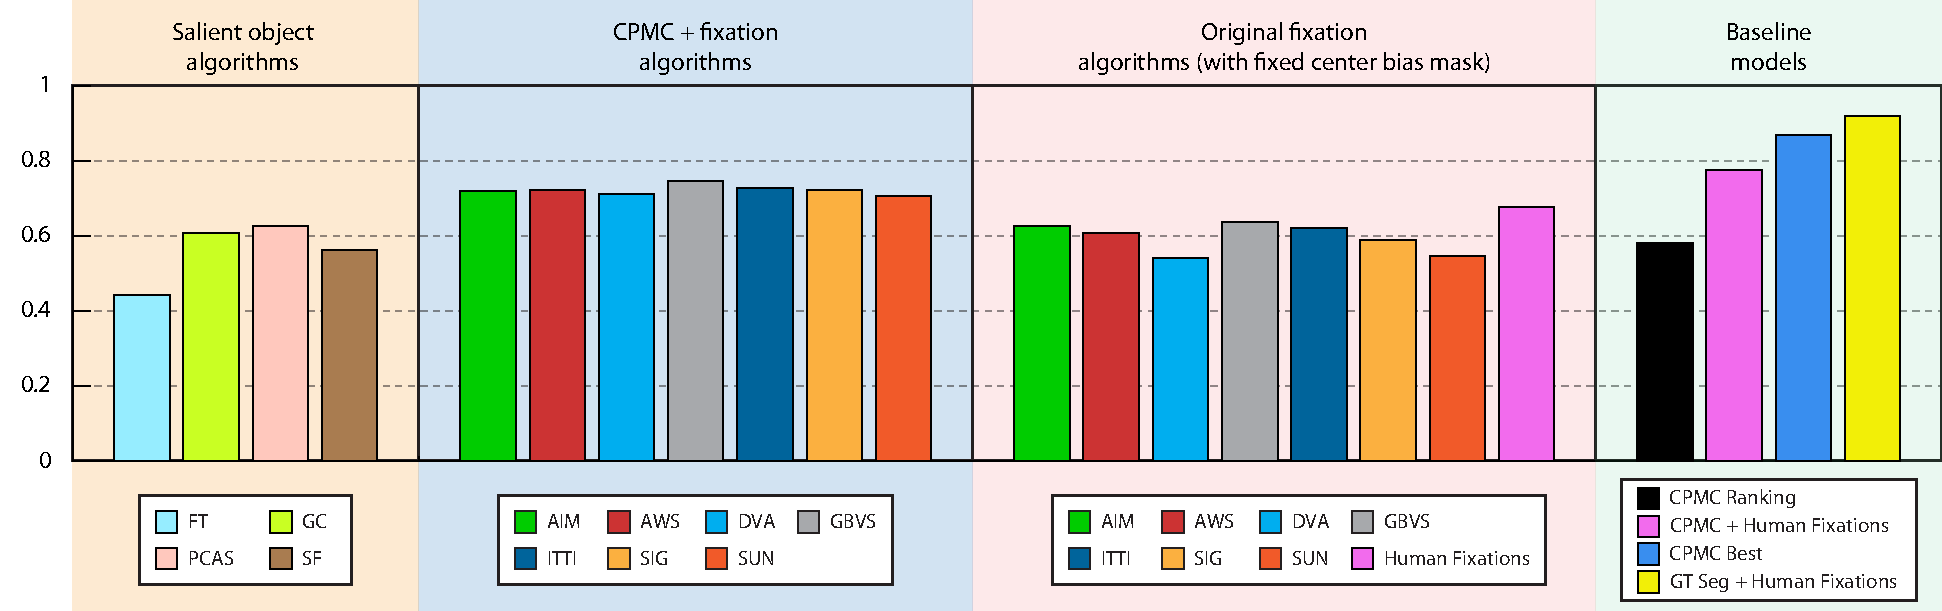
\includegraphics[width=\linewidth]{bigbigFig.pdf}\\
\caption{The F-measures of all algorithms on PASCAL-S dataset.  All CPMC+Fixation results are obtained using top $K=20$ segments.} \label{fig:finalResult}
\end{figure*}

\begin{figure}[htbp]
\centering
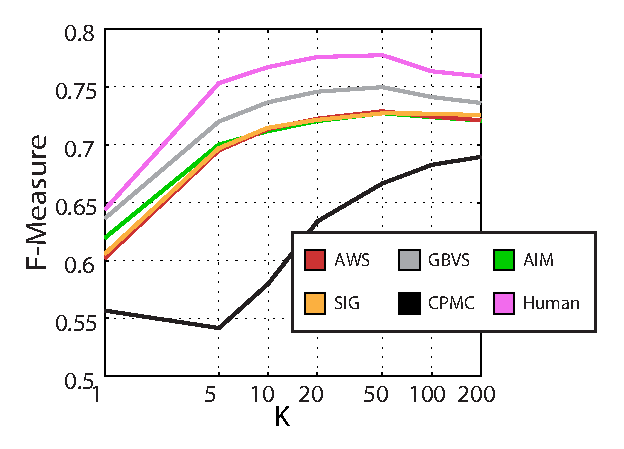
\includegraphics[width=0.6\linewidth]{lastFigCam.pdf}\\
\caption{F-measures of our salient object segmentation method under different choices of $K$, in comparison to CPMC ranking function. Results are reported on the testing set ($60\%$ of the images) of PASCAL-S over 10 random splits. Comparing to the original CPMC ranking function, our method obtains satisfactory F-measures with small $K=20$. } \label{fig:lastFig}
\end{figure}


\begin{table}
\centering
\begin{tabular} {| c | c | c | c || c | c | c | c | }
\hline
\textbf{Salient Object} & FT & IS & PASCAL-S & \textbf{Baseline Models} & FT & IS & PASCAL-S\\
\hline
FT & 0.7427 & 0.4736 & 0.4325 & CPMC Ranking & 0.2661 & 0.3918 & 0.5799\\
\hline
GC & 0.8383 & 0.6261 & 0.6072 & CPMC + Human & N/A & 0.7863 & 0.7756\\
\hline
PCAS & 0.8646 & \textbf{0.6558} & \textbf{0.6275} & CPMC Best & 0.9496 & 0.8416 & 0.8699\\
\hline
SF & \textbf{0.8850} & 0.5555 & 0.557 & GT Seg. + Human & N/A & N/A & 0.9201\\
\hline
\hline
\textbf{Orig. Fixation} & FT & IS & PASCAL-S & \textbf{CPMC + Fixation} & FT & IS & PASCAL-S\\
\hline
AIM & 0.7148 & 0.4522 & \textbf{0.6216} & AIM & 0.8920 & 0.6728 & 0.7204\\
\hline
AWS & \textbf{0.7240} & \textbf{0.6121} & 0.5906 & AWS & 0.8998 & 0.7241 & 0.7224\\
\hline
DVA & 0.6592 & 0.3764 & 0.5223 & DVA & 0.8700 & 0.6377 & 0.7112\\
\hline
GBVS & 0.7093 & 0.5308 & 0.6186 & GBVS & \textbf{0.9097} & \textbf{0.7264} & \textbf{0.7454}\\
\hline
ITTI & 0.6816 & 0.4452 & 0.6079 & ITTI & 0.8950 & 0.6827 & 0.7288\\
\hline
SIG & 0.6959 & 0.5131 & 0.5850 & SIG & 0.8908 & 0.7255 & 0.7214\\
\hline
SUN & 0.6708 & 0.3314 & 0.5281 & SUN & 0.8635 & 0.6249 & 0.7058\\
\hline
\end{tabular}
\caption{The F-measures of all algorithms on all 3 datasets.} \label{tab:fmeasures}
\end{table}

\begin{table}
\begin{center}
\begin{tabular} {l| c c c}
\hline
\hline
K=20                    & PASCAL-S    & IS     & FT \\
\hline
Fixation Model Used     & GBVS      & GBVS    & GBVS\\
F-Measure               & 0.7457    & 0.7264 & 0.9097\\
Improvements            & \textbf{+11.82}    & \textbf{+7.06}  & \textbf{+2.47} \\
\hline
Best SalObj Model       & PCAS      & PCAS   & SF \\
F-Measure               & 0.6275    & 0.6558 & 0.8850 \\
\hline
\hline
\end{tabular}
\caption{Best results of our model compared to best results of existing salient object algorithms.  Our model achieves better F-measure than all major salient object segmentation algorithms on all \textbf{three} datasets, including the heavily biased FT dataset. Results are reported on the testing set ($60\%$ of the images) over 10 random splits in three datasets.} \label{tab:scores}
\end{center}
\end{table}

To better understand our results, we also provide qualitative visualization of salient object masks generated by our methods as well as others. Fig.~\ref{fig:ftRes}-\ref{fig:pascalRes} demonstrate our results using 7 different fixation prediction algorithms in comparison to CPMC ranking function and major salient object segmentation methods, on FT, IS and PARSCAL-S, respectively. We also present our results using human fixations in PASCAL-S and IS.  To illustrate the strength and weakness of our method, we select the results based on the F-measures of each image. For each dataset, the average F-measure of our method decreases from top row to the bottom row. Our method is able to capture the full region of an salient object.  We notice that our method does not segment most of the small salient objects. This is largely due to the output from CPMC using sparse uniform seeds. An object is missing if CPMC does not generate a segment for the object.







%In addition to training and testing within the same dataset, we also investigate the generalization power of our model, by training and testing on different datasets.  The results as F-Measure are shown in Tab.~\ref{tab:crossDataset}.
%\begin{table}
%\begin{center}
%\begin{tabular}{c|c|c|c}
%\hline
%\hline
%\backslashbox{Train}{Test} & FT & IS & PASCAL-S \\
%\hline
%FT & N/A & 0 & 0 \\
%IS & 0 & N/A & 0 \\
%PASCAL-S & 0 & 0 & N/A \\
%\hline
%\hline
%\end{tabular}
%\end{center}
%\caption{Testing the generalization power of the dataset.  We train the random forest based on $50\%$ images from one dataset and benchmark the F-Measure using all images from the other dataset.}\label{tab:crossDataset}
%\end{table}

